\begin{figure}[ht]
\centering
\adjustbox{max width=\linewidth}{
\begin{tikzpicture}[font=\small,
  oplbl/.style={font=\small\ttfamily, anchor=east, minimum width=3.2cm, align=right},
  resnode/.style={font=\small, anchor=west, text=green!40!black}
]

\def\yA{0}
\def\yB{-2.0}
\def\yC{-4.0}
\def\xstart{3.5}
\def\xend{13.5}
\def\tickH{0.12}
\def\SCALE{0.9}

\draw[black!40, line width=0.8pt] (\xstart, \yA) -- (\xend, \yA);
\foreach \x in {0,...,10} {
  \pgfmathsetmacro\xpos{\xstart + \x*\SCALE}
  \draw[black!40] (\xpos, \yA-\tickH) -- (\xpos, \yA+\tickH);
  \node[font=\scriptsize, black!60] at (\xpos, \yA-0.28) {\x};
}

\draw[black!40, line width=0.8pt] (\xstart, \yB) -- (\xend, \yB);
\foreach \x in {0,...,10} {
  \pgfmathsetmacro\xpos{\xstart + \x*\SCALE}
  \draw[black!40] (\xpos, \yB-\tickH) -- (\xpos, \yB+\tickH);
  \node[font=\scriptsize, black!60] at (\xpos, \yB-0.28) {\x};
}

\draw[black!40, line width=0.8pt] (\xstart, \yC) -- (\xend, \yC);
\foreach \x in {0,...,10} {
  \pgfmathsetmacro\xpos{\xstart + \x*\SCALE}
  \draw[black!40] (\xpos, \yC-\tickH) -- (\xpos, \yC+\tickH);
  \node[font=\scriptsize, black!60] at (\xpos, \yC-0.28) {\x};
}

\pgfmathsetmacro\Axs{\xstart+3*\SCALE}
\pgfmathsetmacro\Axe{\xstart+7*\SCALE}
\pgfmathsetmacro\Bxs{\xstart+5*\SCALE}
\pgfmathsetmacro\Bxe{\xstart+9*\SCALE}
\pgfmathsetmacro\Ovs{\xstart+5*\SCALE}
\pgfmathsetmacro\Ove{\xstart+7*\SCALE}

\draw[gray!40, fill=gray!10, line width=0.8pt]
  (\Axs, \yA+0.35) rectangle (\Axe, \yA+0.6);
\node[font=\scriptsize] at ({(\Axs+\Axe)/2}, \yA+0.48) {\texttt{[3,7]}};

\draw[gray!40, fill=gray!10, line width=0.8pt]
  (\Bxs, \yA+0.65) rectangle (\Bxe, \yA+0.9);
\node[font=\scriptsize] at ({(\Bxs+\Bxe)/2}, \yA+0.78) {\texttt{[5,9]}};

\draw[orange!75!black, fill=orange!15, line width=1pt]
  (\Ovs, \yA+0.35) rectangle (\Ove, \yA+0.9);
\node[font=\scriptsize] at ({(\Ovs+\Ove)/2}, \yA+0.63) {overlap};

\pgfmathsetmacro\Cxs{\xstart+2*\SCALE}
\pgfmathsetmacro\Cxe{\xstart+9*\SCALE}
\pgfmathsetmacro\Dxs{\xstart+4*\SCALE}
\pgfmathsetmacro\Dxe{\xstart+6*\SCALE}

\draw[gray!40, fill=gray!10, line width=0.8pt]
  (\Cxs, \yB+0.35) rectangle (\Cxe, \yB+0.9);
\node[font=\scriptsize] at ({(\Cxs+\Cxe)/2}, \yB+0.78) {\texttt{[2,9]} (outer)};

\draw[orange!75!black, fill=orange!15, line width=1pt]
  (\Dxs, \yB+0.38) rectangle (\Dxe, \yB+0.62);
\node[font=\scriptsize] at ({(\Dxs+\Dxe)/2}, \yB+0.50) {\texttt{[4,6]}};

\pgfmathsetmacro\Exs{\xstart+1*\SCALE}
\pgfmathsetmacro\Exe{\xstart+5*\SCALE}
\pgfmathsetmacro\Fxs{\xstart+5*\SCALE}
\pgfmathsetmacro\Fxe{\xstart+9*\SCALE}
\pgfmathsetmacro\Touchx{\xstart+5*\SCALE}

\draw[gray!40, fill=gray!10, line width=0.8pt]
  (\Exs, \yC+0.6) rectangle (\Exe, \yC+0.85);
\node[font=\scriptsize] at ({(\Exs+\Exe)/2}, \yC+0.73) {\texttt{[1,5]}};

\draw[gray!40, fill=gray!10, line width=0.8pt]
  (\Fxs, \yC+0.6) rectangle (\Fxe, \yC+0.85);
\node[font=\scriptsize] at ({(\Fxs+\Fxe)/2}, \yC+0.73) {\texttt{[5,9]}};

\draw[blue!60!black, fill=blue!7, line width=1pt]
  (\Touchx-0.07, \yC+0.55) rectangle (\Touchx+0.07, \yC+0.90);
\node[font=\scriptsize, blue!60!black] at (\Touchx, \yC+1.05) {5};

\node[oplbl] at (\xstart-0.1, \yA+0.6) {\texttt{[3,7] \&\& [5,9]}};
\node[resnode] at (\xend+0.2, \yA+0.6) {\faCheck\ overlap};

\node[oplbl] at (\xstart-0.1, \yB+0.6) {\texttt{[2,9] @> [4,6]}};
\node[resnode] at (\xend+0.2, \yB+0.6) {\faCheck\ contains};

\node[oplbl] at (\xstart-0.1, \yC+0.7) {\texttt{[1,5] -|- [5,9]}};
\node[resnode] at (\xend+0.2, \yC+0.7) {\faCheck\ adjacent};

\end{tikzpicture}
}
\caption{Three range type operators on a number line.}
\end{figure}
